\chapter{I sistemi operazionali}
\thispagestyle{chapterInit}
\label{ch:operazionali}

\section{Finalità dei sistemi operazionali}
    Le principali finalità dei \textbf{sistemi operazionali} riguardano:
    \begin{description}
        \item[Registrazione delle transazioni] Il processo di acquisizione e memorizzazione delle informazioni relative alle transazioni aziendali.
        \item[Pianificazione e controllo] La possibilità di pianificare le operazioni aziendali e controllarne l'effettiva esecuzione.
        \item[Acquisizione ed organizzazione della conoscenza] La possibilità di acquisire e organizzare la conoscenza aziendale.
        \item[Elaborazione delle situazioni aziendali] La possibilità di elaborare le informazioni aziendali per ottenere una visione complessiva della situazione aziendale.
    \end{description}
    Per raggiungere questa finalità il sistema operazionale si compone di due sottosistemi principali:
    \begin{description}
        \item[Base di dati operazionale] Contiene le informazioni operative in forma organizzata.
        \item[Funzioni operative] Sono le funzioni che permettono di acquisire, memorizzare, elaborare e trasmettere le informazioni.
    \end{description}
    \subsection{Transazioni}
        \subsubsection{Cos'è una transazione}
            \paragraph{Definzione} Per definizione una \textbf{transazione} è una operazione detta \textbf{atomica} (ovvero indivisibile) che si manifesta in un certo e conosciuto momento ed è una informazione che l'azienda è interessata a registrare.
            \paragraph{Esempi} Alcuni esempi di transazioni sono: gli ordini tra cliente e fornitori, prelievi da magazzino, spedizioni, pagamenti, ecc\dots
        \subsubsection{Registrazione delle transazioni}
            Le transazioni da dover registrare, possono essere sostanzialmente di due tipi:
            \begin{description}
                \item[Semplici] Si deve registrare nel sistema solo un singolo dato.
                \item[Complesse] Si devono registrare più operazioni elementari connesse in senso logico e spesso corelate a documenti fisici, quali ad esempio una spedizione che è correlata ad una \textit{bolla di spedizione}.
            \end{description}
            Inoltre una transazione può generarle delle altre e quindi si parla di \textbf{transazioni a cascata}.
            \paragraph{Volume dei dati} Ogni transazione produce un volume di dati dipendentemente dalla natura dell'attività e dell'organizzazione aziendale.
    \subsection{Pianificazione e controllo delle operazioni}
        Alcuni processi aziendali sono dipendenti da altri, si rende quindi necessario usare i dati dei processi "a monte" per pianificare e controllare i processi "a valle". Tramite l'uso di \texttt{SI} è possibile adottare modelli più complessi di pianificazione e monitorare continuativamente l'andamento dello stato dei processi aziendali. 
        \paragraph{Perché pianificare e controllare} Pianificare e controllare i processi aziendali ha diversi vantaggi per l'azienda, sia per il passato che per il presente fino ad avere anche una utilità per i processi futuri. Questi vantaggi sono raggiunti tramite: La possibilità di elaborare piani e strategie di produzione, registrare e monitorare l'avanzamento delle operazioni ed infine la possibilità di misurare se e quanto i piani sono stati rispettati rispetto agli obiettivi prefissati.
            \subparagraph{Come pianificare e controllare} Il \texttt{SI} deve essere dotato di funzioni molto articolate e specifiche per l'azienda alla quale si riferisce, ad esempio quando parliamo di "Elaborazione di piani" il \texttt{SI} di riferimento deve essere in grado di: ottimizzare le risorse disponibili, sincronizzare le operazioni ed essere coerente con lo stato degli indicatori aziendali.
    \subsection{Elaborazione delle situazioni aziendali}
        Il \texttt{SI} è un sistema dinamico che serve per modellare la realtà aziendale e per fornire informazioni utili per la gestione aziendale. La conoscenza dello stato corrente, oltre che di quello passato, è fondamentale per la gestione aziendale, questa conoscenza permette di pilotare l'azienda grazie a determinati eventi. Alcuni indicatori di stato sono ad esempio: le giacenze di magazzino, i tempi di consegna, i tempi di produzione, ecc\dots\newline
        Gli indicatori dunque non rappresentano una situazione statica, ma una situazione dinamica che cambia nel tempo. Questi indicatori sono utili per la gestione aziendale e per la pianificazione delle attività future. Tutti gli indicatori di stato sono calcolati a partire dai dati inseriti, modificati e cancellati dalle transazioni aziendali e sono utili per la gestione aziendale.
\section{Informazione Operativa}
    L'informazione operativa è costituita principalmente da archivi nei quali sono presenti relazioni che coinvolgono diverse entità, questi archivi solitamente li classifichiamo in:
    \begin{description}
        \item[Movimenti] Contengono le informazioni relative alle transazioni semplici, relative ad un singolo oggetto.
        \item[Documenti] Contengono le informazioni su transazioni complesse che riguardano una lisa di oggetti (classica tabella) dove in testa troviamo anche una serie di informazioni comune a tutte le righe.
        \item[Informazioni di stato] Ovvero un insieme di indicatori di stato che permettono di avere una visione complessiva della situazione aziendale. Questi possono essere \textit{de-materializzati} e quindi calcolati al momento della richiesta o \textit{materializzati} e quindi calcolati e memorizzati in un archivio.
        \item[Informazioni Anagrafiche] Contengono le informazioni relative alle entità che partecipano alle transazioni, questi non si limitano a contenere solo dati di anagrafica di persone fisiche, ma anche di oggetti, di entità giuridiche, ecc\dots
    \end{description}
    \subsection{Qualità dei dati}
        Per qualità dei dati si fà riferimento allo standard \texttt{ISO 8402-1995} citando: "Il possesso della totalità delle caratteristiche che portano al soddisfacimento delle esigenze espresse o implicite, dell'utente".
        \paragraph{La qualità dei dai}
            Per stabilire un indice di qualità dei dati si possono utilizzare diversi parametri quali:
            \begin{itemize}
                \item Tanto più elevata quanto più il sistema fornisce rappresentazioni degli eventi vicine alla percezione diretta della realtà
                \item La dipendenza dalla struttura del \texttt{SI} è minore quanto più i dati sono indipendenti dalla struttura del sistema
                \item La qualità è diminuita da sottosistemi non integrati e da dati ridondanti
            \end{itemize}
            In sostanza un dato per essere di qualità non deve essere ridondante, deve essere coerente con la realtà e deve essere indipendente dalla struttura del sistema.
        \paragraph{Impatto della qualità dei dati}
            Se all'interno del proprio \texttt{SI} si ha una bassa qualità dei dati, allora si avrà un forte impatto economico/organizzativo tra cui: la difficoltà nell'introduzione di innovazioni tecnologiche (adozione di una nuova tecnologia) e di processo (modificare un processo produttivo), la difficoltà nell'avvio di processi del tipo \textit{data warehousing}, inoltre dal lato umano avere una bassa qualità dei dati può portare a una scarsa soddisfazione degli utenti finali del \texttt{SI} (ovvero quelle persone che utilizzano il \texttt{SI} per svolgere il proprio lavoro).
    \subsection{Informazione Operativa}
        L'informazione operativa è l'informazione che serve per svolgere le attività operative dell'azienda, questa informazione è costituita da dati che vengono acquisiti, memorizzati, elaborati e trasferiti all'interno dell'azienda. Questi dati sono utili per la gestione aziendale e per la pianificazione delle attività future. L'informazione operativa è caratterizzata da:
        \begin{description}
            \item[Aggregazione] I dati sono aggregati in base alle esigenze dell'utente, possono essere:
                \subitem \textbf{Analitici} Se si vuole avere una visione dettagliata di un singolo evento.
                \subitem \textbf{Analitici} Se si vuole avere una visione complessiva di un insieme di eventi, ottenuto aggregando i dati.
            \item[Tempificazione] I dati possono essere temporizzati in base alle esigenze dell'utente, possono essere:
                \subitem \textbf{Puntuale} Se si vuole avere una visione istantanea della situazione aziendale.
                \subitem \textbf{Cumulata} Se si vuole avere una visione della situazione aziendale in un certo periodo di tempo.
            \item[Dimensionalità] Intendiamo come dimensionalità il numero minimo di parametri necessari per estrarre una specifica informazione.
        \end{description}
        Esempio delle caratteristiche dell'informazione operativa:
        \begin{table}[H]
            \centering
            \begin{tabular}{|c|c|c|c|}
                \hline
                & \textbf{Aggregazione} & \textbf{Tempificazione} & \textbf{Dimensionalità} \\
                \hline
                \textbf{Anagrafe} & Analitica & Puntuale & unitaria \\
                \hline
                \textbf{Movimenti \& Documenti} & Analitica & Puntuale & Contenuta \\
                \hline
                \textbf{Informazioni di stato} & Analitica o aggregata & Puntuale o cumulata & Contenuta \\
                \hline
            \end{tabular}
        \end{table}
\section{Potenzialità informatica}
    \paragraph{Definzione} La \textbf{potenzialità informatica} è costituita principalmente da due indicatori:
    \begin{description}
        \item[Intensità informativa] Misura la quantità di informazioni della quale l'azienda necessita, sia che queste vengano da fonti interne o esterne.
        \item[Attrattiva informatica] Ovvero la propensione dell'azienda ad utilizzare un \texttt{SI} per la gestione delle informazioni.
    \end{description}
    Inoltre la propensione del management verso l'investimento sulla infrastruttura informatica è un indicatore di potenzialità informatica. 
    \subsection{Intensità informativa}
        \paragraph{Definzione} L'intensità informativa è costituita da un insieme di fattori quali:
        \begin{itemize}
            \item La complessità dell'attività aziendale: dimensione, area geografica, appartenenza a strutture complesse, livello di diversificazione dei prodotti, dei mercati e delle tecnologie.
            \item L'intensità informativa di prodotto
                \subitem quantità di informazioni proprie degli oggetti prodotti o dei servizi erogati
            \item L'intensità informativa di processo
                \subitem quantità di informazioni necessarie all'avanzamento dei processi aziendali (o generati da questi)
        \end{itemize}
    \subsection{Attrattiva Informatica}
        \paragraph{Definizione} L'attrattiva informatica e un insieme di fattori che concorrono a determinare quanto un processo aziendale sia attrattivo per l'automazione tramite un \texttt{SI}. Questi fattori sono:
        \begin{itemize}
            \item \textbf{Proceduralità}, ovvero il grado di formalizzazione dei processi aziendali
                \subitem Più un processo è formalizzato, più è attrattivo
            \item \textbf{Complessità}, grado di difficoltà delle azioni elementari previste dal processo
                \subitem Meno un processo è complesso e più è attrattivo
            \item \textbf{Ripetitività}: frequenza con cui un processo viene ripetuto
                \subitem Più un processo è ripetuto, più è attrattivo    
            \item \textbf{Volume}: quantità di dati e informazioni elaborate dal processo
                \subitem Alti volumi di dati rendono un processo attrattivo         
        \end{itemize}
\section[Composizione dei \texttt{SI} Operazionali]{Composizione dei sistemi informativi operazionali}
    I \texttt{SI} operazionali sono composti da diversi sotto-sistemi che si occupano di diverse funzioni. Al momento non esiste una classificazione standard dei sotto-sistemi in quanto varia in base all'azienda e al settore di appartenenza. I criteri principali usati per la distinzione tra diversi sotto-sistemi sono: la funzione svolta, il processo aziendale coinvolto, l'architettura tecnologica, ecc\dots
    \subsubsection{Portafoglio Applicativo}
        Definiamo come \textbf{portafoglio applicativo} l'insieme delle applicazioni software che costituiscono il \texttt{SI} operativo, possono essere individuate due aree principali, ovvero il \textbf{portafoglio operativo} e il \textbf{portafoglio istituzionale}.
        \paragraph{Portafoglio Operativo} È costituito da applicazioni informatiche che trattano di processi legati al \textit{core-business} dell'azienda. Questo genere di portafoglio è caratterizzato da una elevata specializzazione ad un settore specifico oltre ad una elevata variabilità tra aziende dello stesso settore di appartenenza. Inoltre questo portafoglio è caratterizzato da una forte verticalizzazione e da una elevata specializzazione delle funzioni implementate.
        \paragraph{Portafoglio istituzionale} È costituito da applicazioni informatiche che trattano di processi a sostegno delle principali attività aziendali. Questo genere di portafoglio è caratterizzato da una elevata attrattiva informatica e da una alta proceduralita (e ripetitività) dei processi. Inoltre questo genere di portafoglio è caratterizzato da una elevata omogeneità tra aziende anche di settori diversi e la poca variabilità tra servizi e prodotti offerti.
    \subsection{Sistema gestionale classico}
        Nel modello del sistema gestionale classico solitamente sono presenti delle isole informatiche autonome e molto specializzate, questo genere di sviluppo è causato principalmente da uno sviluppo incrementale (ovvero lo sviluppo viene eseguito a compartimenti "stagni" uno per volta), da una rigidità delle organizzazioni aziendali, dalla specializzazione dei produttori di software ecc\dots
        \paragraph{Problematiche} Questo genere di sviluppo porta a diverse problematiche quando si discute sulla gestione dei dati, in questo sistema infatti i dati sono ridondanti, disomogenei e spesso incoerenti. Ad aggiungersi a ciò questo genere di gestionale rende difficile avere una visione complessiva dell'azienda.
        \begin{figure}[H]
            \centering
            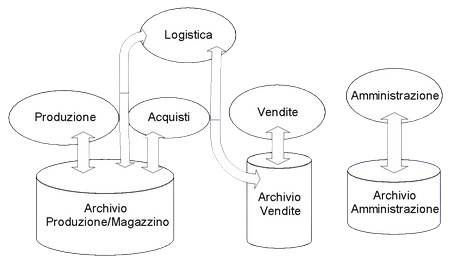
\includegraphics[width=0.5\textwidth]{05/gestionaleClassico.png}
            \caption{Schema dei settori di un sistema gestionale classico}
        \end{figure}
    \subsection{Sistema \texttt{ERP} - \textit{Enterprise Resource Planning}}
        Un sistema \texttt{ERP} è un sistema informativo aziendale integrato, ovvero un sistema che permette di gestire in maniera integrata e coordinata tutte le informazioni aziendali. Questo genere di sistema, grazie ad una basi di dati unica ed a processi integranti e cooperanti, punta a trattare i dati in modo ottimale e ottimizzato, oltre a gestire il controllo dei processi aziendali.
        \paragraph{Vantaggi} Questo genere di sistema così implementato è molto flessibile ed in grado di assecondare l'azienda in ogni sua esigenza, inoltre permette di avere una visione complessiva dell'azienda e di avere una gestione ottimale dei processi aziendali. Inoltre questo si adatta molto rispetto all'organizzazione aziendale e all'architettura tecnologica.
        \begin{figure}[H]
            \centering
            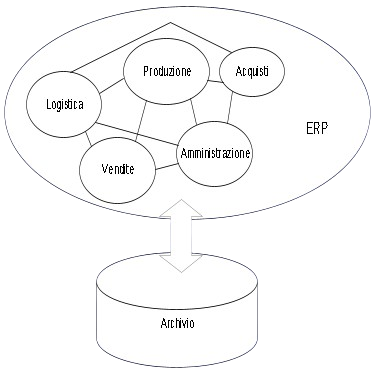
\includegraphics[width=0.33\textwidth]{05/gestionaleERP.png}
            \caption{Schema dei settori di un sistema gestionale \texttt{ERP}}
        \end{figure}
    \subsection{Sistemi operazionali complementari}
        I sistemi operazionali complementari sono sistemi che vengono aggiunti al sistema operativo principale per coprire delle funzioni che non sono presenti nel sistema operativo principale. Questi sistemi sono caratterizzati da una forte specializzazione e da una forte integrazione con il sistema operativo principale.
        \paragraph{Esempi di sistemi operazionali complementari} Alcuni esempi di sistemi operazionali complementari sono: i sistemi di supporto alle decisioni, i sistemi di gestione della qualità, i sistemi di gestione ambientale, le estensioni dell'\texttt{ERP} ecc\dots